\documentclass[xcolor=table]{beamer}


\usepackage[utf8]{inputenc}
\usepackage[spanish, es-tabla, activeacute]{babel}

\usetheme[ pageofpages=of,% String used between the current page and the
                         % total page count.
          bullet=circle,% Use circles instead of squares for bullets.
          titleline=true,% Show a line below the frame title.
          alternativetitlepage=false,% Use the fancy title page.
          titlepagelogo=unl,% Logo for the first page.
          watermark=agua-unl,% Watermark used in every page.
          watermarkheight=90px,% Height of the watermark.
          watermarkheightmult=4,% The watermark image is 4 times bigger
                                % than watermarkheight.
          ]{Torino}

\author{Leandro Ferrado \and Matías Cuenca-Acuna}

\subtitle{}
\title{Filtrando eventos de seguridad en forma conservativa mediante deep learning}

\urldef{\mailsa}\path|{leandro.ferrado, francisco.m.cuenca-acuna}@intel.com|

\institute{Argentina Software Design Center (ASDC), Intel Security - Córdoba, Argentina\\ \mailsa} %\\


\titlegraphic{\includegraphics[height=1cm]{Intel_McAfee_Security}}

\date{5 de Septiembre del 2016}
%-----------------------------------------
% Definición de comandos útiles
\setbeamertemplate{navigation symbols}{}

\makeatletter
\setbeamertemplate{footline}
{
	\leavevmode%
	\hbox{%
		\begin{beamercolorbox}[wd=.3\paperwidth,ht=2.25ex,dp=1ex,center]{date in head/foot}%
			\usebeamerfont{date in head/foot}
			ASDC - Intel Security.
			
		\end{beamercolorbox}%
		\begin{beamercolorbox}[wd=.4\paperwidth,ht=2.25ex,dp=1ex,center]{author in head/foot}%
			\usebeamerfont{author in head/foot}
			ASAI 2016
		\end{beamercolorbox}}%
		\begin{beamercolorbox}[wd=.3\paperwidth,ht=2.25ex,dp=1ex,right]{date in head/foot}%
			\usebeamerfont{date in head/foot}\insertshortdate{}\hspace*{2em}
			\insertframenumber{} / \inserttotalframenumber\hspace*{2ex}
		\end{beamercolorbox}%
		\vskip0pt%
	}
	\makeatother
	
	\date[05/09/16]{\tiny 5 de Septiembre del 2016}
	
	
	\AtBeginSection[]
	{
		\begin{frame}
			\frametitle{Contenidos:}
			\tableofcontents[currentsection]
		\end{frame}
	}

\usepackage{xcolor}


\begin{document}
% DO NOT COMPILE THIS FILE DIRECTLY!
% This is included by the other .tex files.

\begin{frame}[t,plain]
\titlepage
\end{frame}

\begin{frame}
	\frametitle{Contenidos:}
	
	\tableofcontents
\end{frame}

\section{Resumen}
%---------------------------------------
\begin{frame}[t,fragile]
	\frametitle {Resumen}
	\begin{block}{}
		\begin{itemize}
			\item Aprendizaje Profundo
			\pause
			\item Distribuci\'on del c\'omputo
			\pause
			\item Clasificaci\'on en se\~nales de EEG
		\end{itemize}
	\end{block}
\end{frame}
%--------------------------------------- 
\section{Justificaci\'on}
%---------------------------------------
\begin{frame}[t,fragile]{Justificaci\'on}
	\begin{block}{}
		\begin{itemize}
			\item \alert{Problemas complejos} $\Rightarrow$ Aprendizaje profundo
			\pause
			
			\item \alert{Costo computacional} $\Rightarrow$ Sistema distribuido (local - cl\'uster)
			\pause
			
			\item \color{blue}{Reutilizable por desarrolladores}
			\begin{itemize}
				\item Interfaz y documentaci\'on claras
				\item Transparencia del c\'alculo paralelo involucrado
			\end{itemize}
			\pause
						
			\item \color{blue}{Uso de autocodificadores}
			\pause
			
			\item Aplicaci\'on en problem\'atica compleja:
			\begin{itemize}
				\item ''Clasificaci\'on sobre se\~nales cerebrales''
				\item Interfaz cerebro-computadora (ICC)
				\item Comunicaci\'on confiable usando \'epocas \'unicas (single-trial)
			\end{itemize}
			

		\end{itemize}
	\end{block}
\end{frame}
%--------------------------------------- 

%---------------------------------------
\section{Objetivos}
%---------------------------------------
\begin{frame}[t,fragile]{Objetivos generales}
	\begin{block}{}
	
		\begin{itemize}
			\item Desarrollar un framework con algoritmos de aprendizaje profundo para
			entrenamiento y validaci\'on de redes neuronales, con posibilidad de distribuir el
			trabajo computacional sobre una computadora y/o una red de ellas.
			\item Aplicar la implementaci\'on obtenida en problemas de clasificaci\'on sobre datos de
			se\~nales cerebrales, con el fin de analizar la potencialidad de las herramientas
			desarrolladas.
		\end{itemize}
	\end{block}
\end{frame}

\begin{frame}[t,fragile]{Objetivos espec\'ificos}
	\begin{block}{}
		\begin{itemize}
			\item Definir funcionalidades y herramientas del framework.
			%\pause
			\item Investigar e implementar un motor de procesamiento distribuido escalable a cl\'usteres.
			%\pause
			\item Lograr concurrencia para el entrenamiento de redes neuronales profundas a trav\'es
			de los nodos de un cl\'uster.
			%\pause
			\item Obtener un software con c\'odigo suficientemente documentado en todas sus
			funcionalidades.
		\end{itemize}
	\end{block}
\end{frame}
%--------------------------------------- 
\begin{frame}[t,fragile]{Objetivos espec\'ificos}
	\begin{block}{}
		\begin{itemize}
			\item Conseguir una interfaz para que abstraiga el c\'omputo paralelo
			implicado.
			%\pause
			\item Desarrollar un protocolo de experimentaci\'on sobre el caso de aplicaci\'on.
			%\pause
			\item Llevar adelante las pruebas especificadas.
			%\pause
			\item Obtener resultados mejores que el azar sobre los datos tratados.
			%\pause
		\end{itemize}
	\end{block}
\end{frame}
%--------------------------------------- 

\section{Alcance}
\begin{frame}[t,fragile]
	\frametitle {Alcance}
	\begin{enumerate}
		\item Enfoque de autocodificadores para pre-entrenamiento de redes neuronales profundas.
		\pause
		\item Software con estructura simple y c\'odigo f\'acil de leer\\ $\Rightarrow$ Lenguaje: Python
		\pause
		\item Uso de motor de procesamiento distribuido Apache Spark\texttrademark (libre)
		\pause
		\item Distribuci\'on de c\'omputo a nivel local y nivel cl\'uster
		\pause
		\item Bases de datos adquiridas de forma gratuita
		\pause
		\item Se\~nales de EEG ya pre-procesadas (no incluye investigaci\'on de fen\'omeno de estudio)
		
	\end{enumerate}
	
\end{frame}

\section{Metodolog\'ia}
%---------------------------------------
\begin{frame}[t,fragile]
	\frametitle {Metodolog\'ia}
		\textcolor{blue}{\textbf{Ciclo de vida}: Modelo en cascada} (arquitectura estable y requisitos bastantes predefinidos)\ \\ \ \\ 
		\underline{Etapas}
		\pause
		\begin{enumerate}
			\item Estudio estrat\'egico y recolecci\'on de requisitos
			\pause
			\item Dise\~no de propuesta de soluci\'on
			\pause
			\item Obtenci\'on de recursos y del marco te\'orico
			\pause
			\item Producci\'on y testeo del software
			\pause
			\item Puesta en marcha y experimentaci\'on
			\pause
			\item An\'alisis de resultados e informe de trabajo
			
		\end{enumerate}
\end{frame}
%--------------------------------------- 

\section{Cronograma}
%---------------------------------------
\watermarkoff
\begin{frame}[t,fragile]
	\frametitle {Cronograma}
	
	\begin{figure}
		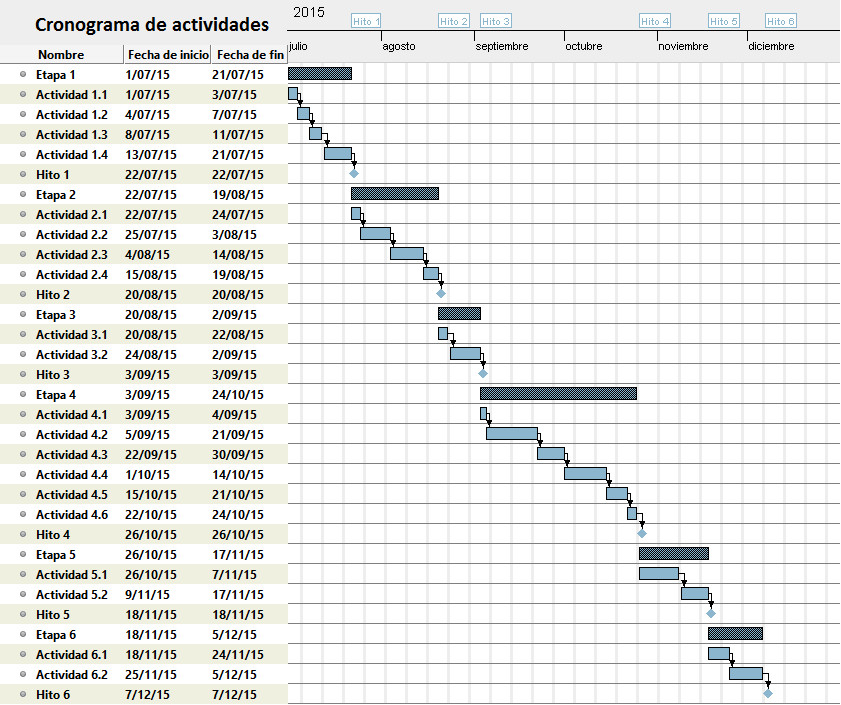
\includegraphics[height=7cm]{imagenes/cronograma.png}
	\end{figure}

\end{frame}
\watermarkon
%--------------------------------------- 

\section{Riesgos}
%---------------------------------------
\watermarkoff
\begin{frame}[t,fragile]
	\frametitle {Riesgos}
	\begin{figure}
		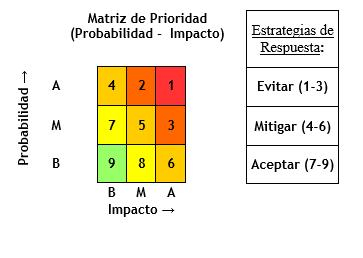
\includegraphics[height=7cm]{imagenes/prioridad.jpg}
	\end{figure}
\end{frame}
\watermarkon
\begin{frame}[t,fragile]
	\frametitle {Riesgos}
	\begin{enumerate}[R001]
		\item \textbf{Incapacidad de integraci\'on del motor de procesamiento distribuido en las actividades de producci\'on del software.}\\
		%\underline{Consecuencia}: Retraso en las actividades de integraci\'on y testeo del software.\\
		%\textit{S\'intoma:} Dificultad de uso del motor y funcionamiento incorrecto durante las pruebas de integraci\'on\\
		\underline{Prioridad}: 6 $\Rightarrow$ \colorbox{yellow!50!orange}{Mitigar probabilidad}
		\pause
		\item \textbf{Incompatibilidades al migrar el trabajo del framework de la PC a los nodos del cl\'uster.}\\
		\underline{Prioridad}: 3 $\Rightarrow$ \colorbox{orange!100}{Evitar}
		\pause
		\item \textbf{Carencia/deficiencia de la base de datos correspondiente al caso de aplicaci\'on elegido.}\\
		\underline{Prioridad}: 6 $\Rightarrow$ \colorbox{yellow!50!orange}{Mitigar probabilidad}
		\pause
		\item \textbf{Inconsistencias que surjan durante la experimentaci\'on, en el comportamiento de las funcionalidades elegidas.}\\
		\underline{Prioridad}: 6 $\Rightarrow$ \colorbox{yellow!50!orange}{Mitigar impacto}			
	\end{enumerate}
\end{frame}


\begin{frame}[t,fragile]
	\frametitle {Riesgos}
	\begin{enumerate}[R001]
		\addtocounter{enumi}{4}
		\item \textbf{Nodos de cl\'usteres no disponibles por el tiempo necesario para completar la experimentaci\'on.}\\
		\underline{Prioridad}: 5 $\Rightarrow$ \colorbox{yellow!50!orange}{Mitigar impacto}
		\pause
		\item \textbf{No disponibilidad del responsable de la ejecuci\'on del proyecto.}\\
		\underline{Prioridad}: 6 $\Rightarrow$ \colorbox{yellow!50!orange}{Mitigar impacto}
		\pause
		\item \textbf{No disponibilidad de los directores del proyecto.}\\
		\underline{Prioridad}: 8 $\Rightarrow$ \colorbox{yellow!100}{Aceptar}
		\pause
		\item \textbf{Experimentaci\'on lenta e insuficiente sobre el caso de aplicaci\'on.}\\
		\underline{Prioridad}: 5 $\Rightarrow$ \colorbox{yellow!50!orange}{Mitigar impacto}			
	\end{enumerate}
\end{frame}
%--------------------------------------- 
\section{Recursos}
%---------------------------------------
\begin{frame}[t,fragile]
	\frametitle {Recursos}
	\begin{block}{}
		\underline{Disponibles}
		\begin{itemize}
			\item Computadora Personal (multi-n\'ucleo)
			\item Bibliograf\'ia (FICH, MinCyT)
			\item Servicios del Proyecto (Internet, electricidad, etc.)
			\pause
		\end{itemize}
		\underline{Necesarios}
		\begin{itemize}
			\item Software (tecnolog\'ias libres)
			\item Bases de datos p/ caso de aplicaci\'on
			\item Servicio de cl\'uster
		\end{itemize}
	\end{block}
\end{frame}
%--------------------------------------- 

\section{Costos}
%---------------------------------------
\begin{frame}[t,fragile]
	\frametitle {Costos}
		\begin{itemize}
			\item Bienes de capital:
			\begin{itemize}
				\item Notebook Asus N56VB S3065H DF Intel Core i5
				\begin{itemize}
					\item Valor a nuevo (VN): \$22000
					\item Valor residual (VR): \$1500
					\item Vida \'util (VU): 12000 horas
					\item Monto de amortizaci\'on:
					 $\frac{VN-VR}{VU} \cdot \text{horas de uso}\approx \textbf{\$697}$
				\end{itemize}
			\end{itemize}
			\pause
			\item Consultor\'ias y Servicios:
			\begin{itemize}
				\item Servicio de cl\'uster computacional (Costos directos):
				\begin{itemize}
					 
					\item 4 nodos por cl\'uster
					\item 4 n\'ucleos por nodo
					\item 7GB de RAM por nodo
					\item 100GB de almacenamiento
					
					Costo: \$3,60/h    
					\textbf{Total \$864.}
				\end{itemize}
			\end{itemize}
		\end{itemize}
\end{frame}
%--------------------------------------- 
\begin{frame}[t,fragile]
	\frametitle {Costos}
		\begin{itemize}
			\item Recursos humanos (Costos directos):
			\begin{itemize}
				\item Remuneraci\'on propia: 
				\begin{itemize}
					\item Rol de analista funcional (Etapas 1, 2, 3 y 6). \\Monto: \$160/h. Total: \textbf{\$34080.} 
					\item Rol de analista programador y tester (Etapas 4 y 5).\\Monto: \$130/h. Total: \textbf{\$25350.} 
					\item \textbf{Total: \$59430.} 		
				\end{itemize}
				\pause
				\item Remuneraci\'on del Director de proyecto:
				\begin{itemize}
					\item Rol de L\'ider de Proyecto. 120hs.
					\\Monto: \$300/h. Total: \textbf{\$36000.} 	
				\end{itemize}
				\pause
				\item Remuneraci\'on del Co-director de proyecto:
				\begin{itemize}
					\item Rol de L\'ider de Proyecto. 88hs.
					\\Monto: \$300/h. Total: \textbf{\$26400.} 	
				\end{itemize}
			\end{itemize}
		
		\end{itemize}
		
\end{frame}
%--------------------------------------- 
\begin{frame}[t,fragile]
	\frametitle {Costos}
	
		\begin{itemize}
			\item Materiales e Insumos (Costos directos):
			\begin{itemize}
				\item Librer\'ia. Total: \textbf{\$620.} 
			\end{itemize}
			\pause
			\item Viajes y Vi\'aticos (Costos directos): 
			\begin{itemize}
				\item Transporte urbano. Total: \textbf{\$1224.}
				\item Merienda. Total: \textbf{\$250.}
			\end{itemize}
			\pause
			\item Otros costos (Costos indirectos): 
			\begin{itemize}
				\item Electricidad. Total: \textbf{\$234.}
				\item Conexi\'on a Internet. Total: \textbf{\$350.}
			\end{itemize}
			\pause
			\item \underline{Presupuesto total}: \textbf{\color{blue}\$126.069}
		\end{itemize}
		
	
\end{frame}
	
\begin{frame}
	\frametitle{\underline{Bibliograf\'ia}:}
	\begin{itemize}
		\item Karau, H. et. al. (2015): ''Learning Spark. Lightning-Fast Big Data Analysis''. O'Reilly Media.\\
		\item Pentreath, N. (2015): ''Machine Learning with Spark''. Packt Publishing.\\
		\item Langtangen, H. (2008): ''Python Scripting for Computational Science''. Springer. Tercera edici\'on.\\
		\item Gonz\'alez-Casta\~neda, E. F., Torres-Garc\'ia, A. A. et al (2014): ''Sonificaci\'on de EEG para la clasificaci\'on de palabras no pronunciadas'' en Research in Computing Science 74. \\
		\item DaSalla, C. et al (2009): ''Single-trial classification of vowel speech imagery using common spatial patterns'' en Neural Networks 22 (9) (pp. 1334-1339).\\
	
		
	\end{itemize}	
\end{frame}

\begin{frame}
	\frametitle{\underline{Bibliograf\'ia}:}
	\begin{itemize}
		\item I. E. Gareis, G. Gentiletti, R. C. Acevedo, H. L. Rufiner (2011): ''Feature extraction on Brain Computer Interfaces using Discrete Dyadic Wavelet Transform: Preliminary results'' en Journal of Physics: Conference Series (IOP), Volume 313, Number 12011 (pp. 1-7). \\
		\item Erhan, D. et al (2010): ''Why does unsupervised pre-training help deep learning?'' en J. Mach. Learn. Res., 11:625-660. 
		\item Bengio, Y (2009): ''Learning deep architectures for AI'' en Foundations and Trends\textregistered in Machine Learning archive.\\
		
	\end{itemize}	
\end{frame}

\begin{frame}
	\frametitle{\underline{Bibliograf\'ia}:}
	\begin{itemize}
		\item Haykin, S. (2009): ''Neural Networks and Learning Machines''. Prentice Hall. Tercera edici\'on.
		\item Bishop, C.M. (1995): ''Neural Networks for Pattern Recognition''. Oxford: Oxford University Press.
		\item Project management institute, inc (2013): “Gu\'ia de los Fundamentos para la Direcci\'on de Proyectos''. PMI Book. Cuarta edici\'on.
		\item Emiliani, F. (1995): ''Proyectos de investigaci\'on cient\'ifica''. UNL-CONICET-ACNL.
		\item Ander Egg, E, Aguilar Ida\~nez, M. (1998): ''C\'omo elaborar un proyecto''. Editorial Lumen.
		
	\end{itemize}	
\end{frame}


	


\end{document}

